\documentclass[a4paper]{article}
\usepackage{cmap}
\usepackage[utf8]{inputenc}
\usepackage[T2A]{fontenc}
\usepackage[english,russian]{babel} 
\usepackage[left=15mm, top=15mm, right=15mm, bottom=42mm, nohead, nofoot]{geometry}
\usepackage{blindtext}  % рыба-текст
\usepackage{graphicx}  % изобржаения
\usepackage{float} % плавающие объекты
\usepackage{wrapfig}  % изобржаения
\usepackage{tikz} % графика
\usepackage{xcolor} % определение цветов
\usepackage{nicefrac} % красивые дроби
\usepackage{cancel} % сокращение
\usepackage{amsmath,amsfonts,amssymb} % математический пакет
\usepackage{hyperref}  % гиперссылки
\usepackage{fancybox,fancyhdr} % хедер и футер
\usepackage{listings} % код
\pagestyle{fancy}
\fancyhf{}
\fancyhead[L]{Лабораторная работа №1}
\fancyhead[R]{\textit{Ряды Фурье}}
\fancyfoot[C]{\thepage}
\headsep=8mm
\footskip=20mm

\definecolor{urlcolor}{HTML}{3454D1}
\definecolor{linkcolor}{HTML}{3454D1}
\hypersetup{pdfstartview=FitH, linkcolor=linkcolor, urlcolor=urlcolor, colorlinks=true}

\definecolor{strings}{rgb}{0,0.6,0}
\definecolor{comments}{rgb}{0,0.3,0}
\definecolor{numbers}{rgb}{0.5,0.5,0.5}
\definecolor{keywords}{rgb}{0.09,0.61,0.95}
\definecolor{background}{rgb}{0.97,0.97,0.97}
\lstdefinestyle{codestyle}{
    backgroundcolor=\color{background},
    commentstyle=\color{comments},
    keywordstyle=\color{keywords},
    stringstyle=\color{strings},
    numberstyle=\tiny\color{numbers},
    basicstyle=\ttfamily\footnotesize,
    breakatwhitespace=false,
    breaklines=true,
    captionpos=b,
    inputencoding=utf8,
    keepspaces=true,
    numbers=left,
    numbersep=5pt,
    showspaces=false,
    showstringspaces=false,
    showtabs=false,
    tabsize=2,
    extendedchars=true,
    literate=
    {а}{{\cyra}}1
    {б}{{\cyrb}}1
    {в}{{\cyrv}}1
    {г}{{\cyrg}}1
    {д}{{\cyrd}}1
    {е}{{\cyre}}1
    {ж}{{\cyrzh}}1
    {з}{{\cyrz}}1
    {и}{{\cyri}}1
    {й}{{\cyrishrt}}1
    {к}{{\cyrk}}1
    {л}{{\cyrl}}1
    {м}{{\cyrm}}1
    {н}{{\cyrn}}1
    {о}{{\cyro}}1
    {п}{{\cyrp}}1
    {р}{{\cyrr}}1
    {с}{{\cyrs}}1
    {т}{{\cyrt}}1
    {у}{{\cyru}}1
    {ф}{{\cyrf}}1
    {х}{{\cyrh}}1
    {ц}{{\cyrc}}1
    {ч}{{\cyrch}}1
    {ш}{{\cyrsh}}1
    {щ}{{\cyrshch}}1
    {ъ}{{\cyrhrdsn}}1
    {ы}{{\cyrery}}1
    {ь}{{\cyrsftsn}}1
    {э}{{\cyrerev}}1
    {ю}{{\cyryu}}1
    {я}{{\cyrya}}1
    {А}{{\CYRA}}1
    {Б}{{\CYRB}}1
    {В}{{\CYRV}}1
    {Г}{{\CYRG}}1
    {Д}{{\CYR96}}1
    {Е}{{\CYRE}}1
    {Ж}{{\CYRZH}}1
    {З}{{\CYRZ}}1
    {И}{{\CYRI}}1
    {Й}{{\CYRISHRT}}1
    {К}{{\CYRK}}1
    {Л}{{\CYRL}}1
    {М}{{\CYRM}}1
    {Н}{{\CYRN}}1
    {О}{{\CYRO}}1
    {П}{{\CYRP}}1
    {Р}{{\CYRR}}1
    {С}{{\CYRS}}1
    {Т}{{\CYRT}}1
    {У}{{\CYRU}}1
    {Ф}{{\CYRF}}1
    {Х}{{\CYRH}}1
    {Ц}{{\CYRC}}1
    {Ч}{{\CYRCH}}1
    {Ш}{{\CYRSH}}1
    {Щ}{{\CYRSHCH}}1
    {Ъ}{{\CYRHRDSN}}1
    {Ы}{{\CYRERY}}1
    {Ь}{{\CYRSFTSN}}1
    {Э}{{\CYREREV}}1
    {Ю}{{\CYRYU}}1
    {Я}{{\CYRYA}}1
}

\lstset{style=codestyle}

\addto\captionsrussian{
  \renewcommand{\contentsname}
    {\centering Содержание}
}
\newcommand{\section}[1]{
    \phantomsection
    \addcontentsline{toc}{section}{#1}
    \section*{\centering #1}
}
\newcommand{\subsection}[1]{
    \phantomsection
    \addcontentsline{toc}{subsection}{#1}
    \subsection*{\centering #1}
}
\newcommand{\subsubsection}[1]{
    \phantomsection
    \addcontentsline{toc}{subsubsection}{#1}
    \subsubsection*{\centering #1}
}

\newlength{\tempheight}
\newcommand{\Let}{
\mathbin{\text{\settoheight{\tempheight}{\mathstrut}\raisebox{0.4\pgflinewidth}{
\tikz[baseline=0.5ex,line cap=round,line join=round] \draw (0,0) --++ (0.3em,0) --++ (0,2.3ex) --++ (-0.3em,0);
}}}}
\newcommand*\squared[1]{\tikz[baseline=(char.base)]{
            \node[shape=rectangle,draw,inner sep=4pt] (char) {#1};}}
\newcommand*\msquared[1]{\tikz[baseline=(char.base)]{
            \node[shape=rectangle,draw,inner sep=4pt] (char) {$\displaystyle #1$};}}
\newcommand{\at}{\biggr\rvert}
\newcommand{\shiftright}[3]{\makebox[#2][r]{\makebox[#1][l]{#3}}}
\newcommand{\e}{\;\text{e}}
\let\oldint\int
\def\int{\oldint\limits}
\DeclareRobustCommand{\divby}{%
  \mathrel{\vbox{\baselineskip.65ex\lineskiplimit0pt\hbox{.}\hbox{.}\hbox{.}}}%
}

\newcommand\NB{\textbf{N\kern-0.32em\textcolor{red}{B}}}

\begin{document}

\begin{titlepage}
    \begin{center}
        Федеральное государственное автономное образовательное \\ учреждение высшего образования \\[6pt]
        САНКТ-ПЕТЕРБУРГСКИЙ НАЦИОНАЛЬНЫЙ \\ ИССЛЕДОВАТЕЛЬСКИЙ УНИВЕРСИТЕТ ИТМО \\[16pt]
        Факультет систем управления и робототехники \\[26em]
        Лабораторная работа №1 \\[0.5em]
        \textbf{РЯДЫ ФУРЬЕ}
    \end{center}\,\\[10em]
    \begin{flushright}
        Студент: Заводин Е.Ю.\\
        Поток: ЧастМет R23 1.6 \\[0.5em]
        Преподаватели: Перегудин А.А.\\
        Догадин Е.В.
    \end{flushright}\,\\[6em]
    \begin{center}
        {\small Санкт-Петербург \\ 2025}
    \end{center}
\end{titlepage}
\setcounter{page}{2}
\tableofcontents\newpage
\section{Вещественные функции}\

Любую (с некоторыми оговорками в виде условий Дирихле, Дини...) функцию $f(t)$ можно представить в виде бесконечной суммы тригонометрических функций $sin(t)$, $cos(t)$, и $1$, являющихся базисными, при этом такое представление будет называться разложением в ряд Фурье. В общем виде для промежутка длиной $T$ ряд Фурье выглядит так:

$$f(t) = \frac{a_0}{2} + \sum_{n=1}^{\infty} \left( a_n\cos(\omega_nt) + b_n\sin(\omega_nt) \right)\text{, где }\omega_n = \frac{2\pi n}{T}$$\

Функции $\sin(\omega_nt)$ и $\cos(\omega_nt)$ попарно ортогональны, а значит, являются базисными, на любом промежутке длины $T$. Коэффициенты $a_n$ и $b_n$ регулируют косинусы и синусы так, чтобы они сходились в пределе к исходной функции $f(t)$. Сами коэффициенты вычисляются с помощью исходной функции следующим образом:
$$a_n = \frac{2}{T}\int_{h}^{h+T} f(t)\cos\omega_nt\,dt\ \Rightarrow\ a_0 = \frac{2}{T}\int_{x_0}^{x_0+T} f(x)\,dt$$
$$b_n = \frac{2}{T}\int_{h}^{h+T} f(t)\sin\omega_nt\,dt\quad (b_0 = 0)$$\,\\[0.2em]
$$c_n = \frac{1}{T} \int_{h}^{h+T}f(t) e^{-i\omega_nt}\,dt = \frac{1}{T} \int_{h}^{h+T}\left(f(t) \cos{\omega_nt} - f(t) i\sin{\omega_nt}\right)\,dt$$
В ходе выполнения этой лабораторной работы предстоит построить ряд Фурье для периодической функции, заданной кусочно ("квадратной волны"), для чётной и нечётной функций, и для любой периодической функции, состоящей не только из прямых линий и являющейся ни чётной, ни нечётной.

\subsection{Квадратная волна}\

Пусть $a = 2, b = 3, t_0 = 4, t_1 = 5, t_2 = 6$, тогда функция из задания:

$$f(t) = \begin{cases}
    2, & t \in [4, 5), \\
    3, & t \in [5, 6).
\end{cases}$$\

По аналогии с примером из лекции расширим функцию на всё множество действительных чисел, чтобы не умалять общность разложения в ряды Фурье и показать график, охватывающий не менее пары периодов:

\begin{figure}[H]
    \centering \includegraphics[width=0.7\textwidth]{square_wave/func.png}
    \caption{График функции $f(t)$}
\end{figure}\noindent\

Период данной функции равен $T = t_2-t_0= 2 \ \Rightarrow\  \omega_n = \frac{2\pi n}{2}=\pi n$. Найдём коэффициенты Фурье для этой функции --- вычислим первые три $a_n$, $b_n$ и $c_n$ вручную, затем воспользуемся кодом.\

\subsubsection{Ручной расчёт}\

Кусочность функции доставляет немного проблем - необходимо разложить интегралы на два: первый от $t_0$ до $t_1$, второй от $t_1$ до $t_2$, но при этом длина $T$ в $\omega_n$ сохраняется для обоих интегралов.\\[0.5em]

При поиске коэффициентов $a_n$ можно заметить, что косинус - функция чётная, а $f(x)$ --- нечётная, значит, все $a_n$ будут равны нулю.\

Однако можно найти $a_0$:

$$
a_0 = \frac{2}{2}\left( \int_{4}^{5} 2 \cos{0}\,dt + \int_{5}^{6} 3\cos{0}\,dt \right) = \left(\int_{4}^{5} 2\,dt + \int_{5}^{6} 3\,dt\right) = 2t\at^5_4 + 3t\at^6_5 = 10 - 8 + 18 - 15 = 5
$$

Для вычисления коэффициентов $b_n$ найдём, как меняется $b$ в зависимости от $n$:

$$b_n = \frac{2}{2}\left( \int_{4}^{5} 2\sin\frac{2\pi n t}{2}\,dt + \int_{5}^{6} 3\sin\frac{2\pi n t}{2}\,dt\right) = \left( \int_{4}^{5} 2\sin{\pi nt}\,dt + \int_{5}^{6} 3\sin{\pi nt}\,dt\right) = $$
$$= \left( \frac{2\cos{\pi nt}}{\pi nt} \at^5_4 + \frac{3\cos{\pi nt}}{\pi nt}\at^6_5 \right) = \left( \frac{2\cos{4\pi n}}{\pi n} - \frac{2\cos{5\pi n}}{\pi n} + \frac{3\cos{5\pi n}}{\pi n} - \frac{3\cos{6\pi n}}{\pi n}\right)=$$
$$=\frac{1}{\pi n} \left( 2\cos{4\pi n} - 2\cos{5\pi n} + 3\cos{5\pi n} - 3\cos{6\pi n}\right)
$$

$b_1, b_2$ вычислим по найденной выше формуле, чтобы не пересчитывать интегралы:

$$
b_1 = \frac{1}{\pi} \left( 2\cos{4\pi} - 2\cos{5\pi} + 3\cos{5\pi} - 3\cos{6\pi}\right)=\frac{1}{\pi}\left( 2 + 2 - 3 -3 \right) = -\frac{2}{\pi}
$$

$$
b_2 = \frac{1}{2\pi} \left( 2\cos{8\pi} - 2\cos{10\pi} + 3\cos{10\pi} - 3\cos{12\pi}\right)=\frac{1}{2\pi}\left( 2 - 2 + 3 - 3 \right) = 0
$$

Заметно, что $b_n=0$ при всех чётных $n$, при нечётных при возрастании $n$ будет убывать со скоростью $\approx\frac{1}{n}$.

Ищем коэффициенты $c_n$:

$$c_0 = \frac{1}{2}\left( \int_{4}^{5} 2e^{-i\pi0t}\,dt + \int_{5}^{6} 3e^{-i\pi0t}\,dt \right) = \frac{1}{2}\left( \int_{4}^{5} 2\,dt + \int_{5}^{6} 3\,dt \right) = \frac{a_0}{2} = 2.5$$\
$$c_n = \frac{1}{2}\left( \int_{4}^{5}2\cos{\p int} + \int_{5}^{6} 3\cos{\pi nt} \right) - \frac{i}{2}\left( \int_{4}^{5} 2\sin{\pi nt}\,dt + \int_{5}^{6} 3\sin{\pi nt}\,dt \right) = \frac{a_n}{2} - \frac{ib_n}{2} = \frac{1}{2} \cdot 0 - \frac{ib_n}{2} = - \frac{i}{2} b_n$$

Из свойства $c_n=\overline{c_{-n}}$ для вещественных функций становится понятна формула для расчёта $c$ при $n < 0: c_{-n}=\frac{i}{2} b_n$ (или просто сопряжённое к $c_n$...)

$$
c_1 = - \frac{i}{2} \cdot b_1 = \frac{i}{\pi} \text{, откуда } c_{-1} = -\frac{i}{\pi}
$$
$$
c_{2} = - \frac{i}{2} \cdot b_2 = 0 \text{, откуда } c_{-2} = 0
$$
\subsubsection{Код}\

Напишем программу, которая вычисляет коэффициенты Фурье для любого $n$.\

\begin{lstlisting}[language=Python, caption=Вычисление коэффициентов Фурье для кусочной функции]
import numpy as np
import matplotlib.pyplot as plt


def scalar_product(f, g, a, b):
    """
    Вычисляет скалярное произведение функций f и g на интервале [a, b].

    :param f: Функция f(x)
    :param g: Функция g(x)
    :param a: Левая граница интервала
    :param b: Правая граница интервала
    :return: Скалярное произведение функций f и g на интервале [a, b]
    """
    x = np.linspace(a, b, 1000)  # Генерируем точки на интервале [a, b]
    dx = x[1] - x[0]  # Шаг интегрирования
    return np.dot(f(x), g(x)) * dx  # Скалярное произведение функций


def fourier_coefficients(f, a, b, T, n):
    """
    Вычисляет коэффициенты Фурье a_n, b_n и c_n для функции f(t) на интервале [a, b].

    :param f: Функция f(t)
    :param a: Начало интервала
    :param b: Конец интервала
    :param n: Порядок коэффициента
    :return: (a_n, b_n, c_n)
    """
    a_n = (2 / T) * scalar_product(f, lambda t: np.cos(2 * n * np.pi * t / T), a, b)
    b_n = (2 / T) * scalar_product(f, lambda t: np.sin(2 * n * np.pi * t / T), a, b)
    c_n = (1 / T) * scalar_product(f, lambda t: np.exp(-1j * 2 * n * np.pi * t / T), a, b)
    return a_n, b_n, c_n


def func(t):
    return 2 if t % 2 < 1 else 3


if __name__ == "__main__":
    f = np.vectorize(func)  # Исследуемая функция
    T = 2
    a = -T / 2  # Начало интервала
    b = a + T  # Конец интервала
    N = int(input('Введите желаемый N: '))  # Порядок коэффициента

    coeff_names = ['a', 'b', 'c']
    coeffs = []
    for i in range(0, N + 1):
        coefficients_n = fourier_coefficients(f, a, b, T, i)
        coeffs.append(coefficients_n)
        for p in range(len(coeff_names)):
            print(coeff_names[p] + f"_{i}: ", np.round(coefficients_n[p], 3))
        print('\n')
\end{lstlisting}\

Первые три коэффициента Фурье для первой кусочно-заданной функции, вычисленные программно:
\begin{lstlisting}[language=Python, caption=Вычисление коэффициентов Фурье для кусочной функции]
a_0:  5.0       a_1:  0.0       a_2:  0.0
b_0:  0.0       b_1:  -0.637    b_2:  0.0
c_0:  (2.5+0j)  c_1:  0.318j    c_2:  -0j
c_-0:  (2.5-0j)  c_-1:  -0.318j    c_-2:  0j
\end{lstlisting}

Полученные коэффициенты совпали с теми, что были вычислены вручную, и равенство $c_n=\overline{c_{-n}}$ выполняется.
 
\subsubsection{Визуализация квадратного}\

Воспользуемся этими коэффициентами для построения графиков тригонометрического $F_n$ и экспоненциального $G_n$ рядов Фурье для функции $f(t)$:\

\begin{lstlisting}[language=Python, caption=Построение частичных сумм рядов $f$ и их графиков]
    # Разложение через синусы и косинусы
    f_sincos = a[0] / 2 + sum(
        a[n] * np.cos(2 * np.pi * n * t_values / T) + b[n] * np.sin(2 * np.pi * n * t_values / T)
        for n in range(1, N + 1)
    )

    # Разложение через экспоненты
    f_exp = sum(
        c[n] * np.exp(1j * 2 * np.pi * n * t_values / T)
        for n in range(-N, N + 1)
    )

    # Графики
    plt.plot(t_values, f_sincos, label=f"$F_{{{N}}}(t)$", linestyle='dashed', color='red')
    plt.plot(t_values, f_exp, label=f"$G_{{{N}}}(t)$", linestyle='dotted', color='blue')
\end{lstlisting}

\begin{figure}[H]
    \begin{minipage}{0.5\textwidth}
        \centering \includegraphics[width=\textwidth]{square_wave/1.png}
        \caption{$n = 1$}
    \end{minipage}\hfill
    \begin{minipage}{0.5\textwidth}
        \centering \includegraphics[width=\textwidth]{square_wave/2.png}
        \caption{$n = 2$}
    \end{minipage}\\[1em]
    \begin{minipage}{0.5\textwidth}
        \centering \includegraphics[width=\textwidth]{square_wave/5.png}
        \caption{$n = 5$}
    \end{minipage}\hfill
    \begin{minipage}{0.5\textwidth}
        \centering \includegraphics[width=\textwidth]{square_wave/10.png}
        \caption{$n = 10$}
    \end{minipage}\\[1em]
    \begin{minipage}{0.5\textwidth}
        \centering \includegraphics[width=\textwidth]{square_wave/50.png}
        \caption{$n = 50$}
    \end{minipage}
    \begin{minipage}{0.5\textwidth}
        \centering \includegraphics[width=\textwidth]{square_wave/100.png}
        \caption{$n = 100$}
    \end{minipage}
\end{figure}\noindent\

Из приведённых графиков заметно, что ряды Фурье $F_n(t)$ и $G_n(t)$ совпадают и довольно близко приближаются к заданной функции уже при $n = 10$, а при $n=100$ становятся предельно близки к аппроксимируемой функции. Проверим равенство Парсеваля ($|f(t)|^2=\sum_{i=1}^{n} (a_i^2+b_i^2)=\sum_{i=1}^{n} c_i^2$) при $n = 100$ для подтверждения наблюдений:
\begin{lstlisting}[caption={Равенство Парсеваля при $n=100$}, numbers=none]
| |f|^2 - sum(|a_i|^2 + |b_i|^2) | = 0.02229
| |f|^2 - sum(|c_i|^2) |           = 0.02229
\end{lstlisting}

Как и следовало ожидать, отклонение рядов от оригинальной функции довольно низко при выбранном $n$, значит, действительно --- при $n\Rightarrow\infty$ ряд Фурье сойдётся к функции.\\[0.5em]

\subsection{Чётная функция}\

В качестве чётной периодической функции была взята следующая $f(t)$:
$$f(t) = \operatorname{sgn}(\cos t) \cdot \operatorname{sgn}(\cos 2t)\text{, где }sgn(x) = \begin{cases}
    -1, & x < 0, \\
    0, & x = 0, \\
    1, & x > 0.
\end{cases}$$\


График этой функции:
\begin{figure}[H]
    \centering \includegraphics[width=0.7\textwidth]{even_func/func.png}
    \caption{График функции $f(t)$}
\end{figure}\noindent

\subsubsection{Вычисления}\

Период функции $f(t)$ равен $T = 2\pi \ \Rightarrow\  \omega_n = n$. Функция чётная, значит, все коэффициенты $b_n$ будут равны нулю, а $a_n$ и $c_n$ могут быть найдены по следующим формулам:
$$a_n = \frac{2}{2 \pi}\int_{-\pi}^{\pi} \operatorname{sgn}(\cos t) \operatorname{sgn}(\cos 2t)\cos{nt}\,dt   \qquad    c_n = \frac{1}{2\pi}\int_{-\pi}^{\pi}\operatorname{sgn}(\cos t) \operatorname{sgn}(\cos 2t)\exp^{-int}\,dt$$

Изменим программу, которая вычисляет коэффициенты Фурье самостоятельно для любого $n$, под нашу функцию.
\begin{lstlisting}[language=Python, caption={Вычисление коэффициентов Фурье для функции $\operatorname{sgn}(\cos t) \cdot \operatorname{sgn}(\cos 2t)$}]
...

f = np.vectorize(lambda t: np.sign(np.cos(t)) * np.sign(np.cos(2*t)))  # Исследуемая функция

...   
\end{lstlisting}\

Получаем первые три коэффициента разложения Фурье, из которых становится видно, что, действительно, коэффициенты $b_n$ равны нулю:
\begin{lstlisting}[caption=Вывод программы]
a_0:  0.0   a_1:  0.527      a_2:  0.0
b_0:  0.0   b_1:  0.0        b_2:  0.0
c_0:  0j    c_1:  (0.264-0j) c_2:  0j
c_-0:  -0j    c_-1:  (0.264+0j) c_-2:  -0j
\end{lstlisting}\

\subsubsection{Визуализация чётного}\

\begin{figure}[H]
    \begin{minipage}{0.5\textwidth}
        \centering \includegraphics[width=\textwidth]{even_func/1.png}
        \caption{$n = 1$}
    \end{minipage}\hfill
    \begin{minipage}{0.5\textwidth}
        \centering \includegraphics[width=\textwidth]{even_func/2.png}
        \caption{$n = 2$}
    \end{minipage}\\[2em]
    \begin{minipage}{0.5\textwidth}
        \centering \includegraphics[width=\textwidth]{even_func/5.png}
        \caption{$n = 5$}
    \end{minipage}\hfill
    \begin{minipage}{0.5\textwidth}
        \centering \includegraphics[width=\textwidth]{even_func/10.png}
        \caption{$n = 10$}
    \end{minipage}
\end{figure}
\begin{figure}[H]
    \begin{minipage}{0.5\textwidth}
        \centering \includegraphics[width=\textwidth]{even_func/50.png}
        \caption{$n = 50$}
    \end{minipage}
    \begin{minipage}{0.5\textwidth}
        \centering \includegraphics[width=\textwidth]{even_func/100.png}
        \caption{$n = 100$}
    \end{minipage}
\end{figure}\noindent\

Графики частичных рядов хорошо приближают функцию, начиная с $n=5$, а с $n=50$ разница становится минимальна, если не брать в расчёт эффект Гиббса --- около точек разрыва отклонение остаётся заметным даже при больших $n$.\\[0.5em]
Проверим равенство Парсеваля при $n = 100$:
\begin{lstlisting}[caption={Равенство Парсеваля при $n=100$}, numbers=none]
| |f|^2 - sum(|a_i|^2 + |b_i|^2) | = 0.00064
| |f|^2 - sum(|c_i|^2) |           = 0.00064
\end{lstlisting}

\subsection{Нечётная функция}\

В качестве подопытной нечётной функции была выбрана $f(t)=sin(t)^3$, её период $T=2\pi$. 

\begin{figure}[H]
    \centering \includegraphics[width=0.831\textwidth]{odd_func/func.png}
    \caption{График функции $f(t)$}
\end{figure}\noindent

\subsubsection{Вычисления}\

Период функции $f(x)$ равен $T = 2\pi \ \Rightarrow\  \omega_n = n$. Коэффициенты разложения Фурье могут быть найдены следующим образом:

$$b_n = \frac{1}{\pi}\int_{0}^{2\pi} \sin(t)^3 \cos{(nt)}\,dt,
c_n = \frac{1}{2\pi}\int_{0}^{2\pi} \sin(t)^3 \exp^-int\,dt
$$

Все $a_n$ будут равны $0$, так как функция нечётная, поэтому формула для их расчёта не приведена.

Изменим программу, которая вычисляет коэффициенты Фурье самостоятельно для любого $n$, под нашу функцию.
\begin{lstlisting}[language=Python, caption={Вычисление коэффициентов Фурье для функции $f(x)$}]
...

def f(x):
    """Функция, для которой вычисляются коэффициенты Фурье."""
    return np.vectorize(lambda x: np.sin(t) ** 3)

...   
\end{lstlisting}\

Результаты программного вычисления первых трёх коэффициентов разложения Фурье:
\begin{lstlisting}[caption=Вывод программы]
a_0:  0.0       a_1:  0.0           a_2:  -0.0
b_0:  0.0       b_1:  0.75          b_2:  0.0
c_0:  (-0+0j)   c_1:  (-0-0.375j)   c_2:  0j
\end{lstlisting}
Коэффициенты $a_n$ равны нулю и для бОльших $N$, чем приведённые, что говорит о том, что интервал для разложения выбран верно.
\subsubsection{Визуализация нечётного}\
\begin{figure}[H]
    \begin{minipage}{0.5\textwidth}
        \centering \includegraphics[width=\textwidth]{odd_func/1.png}
        \caption{$n = 1$}
    \end{minipage}\hfill
    \begin{minipage}{0.5\textwidth}
        \centering \includegraphics[width=\textwidth]{odd_func/2.png}
        \caption{$n = 2$}
    \end{minipage}
    \begin{minipage}{0.5\textwidth}
        \centering \includegraphics[width=\textwidth]{odd_func/3.png}
        \caption{$n = 3$}
    \end{minipage}\hfill
    \begin{minipage}{0.5\textwidth}
        \centering \includegraphics[width=\textwidth]{odd_func/5.png}
        \caption{$n = 5$}
    \end{minipage}
\end{figure}
\begin{figure}[H]
    \begin{minipage}{0.5\textwidth}
        \centering \includegraphics[width=\textwidth]{odd_func/10.png}
        \caption{$n = 10$}
    \end{minipage}
    \begin{minipage}{0.5\textwidth}
        \centering \includegraphics[width=\textwidth]{odd_func/50.png}
        \caption{$n = 50$}
    \end{minipage}
\end{figure}\noindent\

Ряды Фурье очень быстро сходятся к аппроксимируемой функции за счёт того, что исходная функция --- просто степень синуса, одной из базисных функций разложения Фурье.\\[0.5em]\

Благодаря проверке равенства Парсеваля можно убедиться в том, что при $n=3$ ряды Фурье очень близко приближаются к функции, а при $n=50$ неотличимы от функции к некотором приближении:\\
\begin{minipage}{0.49\textwidth}
\begin{lstlisting}[caption={Равенство Парсеваля при $n=3$}]
| |f|^2 - sum(|a_i|^2 + |b_i|^2) | = 0.01685
| |f|^2 - sum(|c_i|^2) |           = 0.01685
\end{lstlisting}
\end{minipage}\hfill
\begin{minipage}{0.48\textwidth}
\begin{lstlisting}[caption={Равенство Парсеваля при $n=50$}, numbers=none]
| |f|^2 - sum(|a_i|^2 + |b_i|^2) | = 0.00000
| |f|^2 - sum(|c_i|^2) |           = 0.00000
\end{lstlisting}
\end{minipage}\

\subsection{Ни рыба, ни мясо}\

В этом случае взята функция $((x\mod{1}))^2$ на отрезке $[0,1]$ с длиной периода $T=1$:
\begin{figure}[H]
    \centering \includegraphics[width=0.7\textwidth]{periodic_func/func.png}
    \caption{График функции $f(x)$}
\end{figure}\noindent\

Период функции $f(x)$ равен $T = 1 \ \Rightarrow\  \omega_n = 2\pi n$. Коэффициенты разложения Фурье могут быть найдены следующим образом:
$$a_n = \frac{1}{\pi}\int_{0}^{2\pi} \left(\frac{x}{\pi} \bmod 2\right)^2\sin nx\,dx\qquad b_n = \frac{1}{\pi}\int_{0}^{2\pi} \left(\frac{x}{\pi} \bmod 2\right)^2\cos nx\,dx\qquad c_n = \frac{1}{2\pi}\int_{0}^{2\pi}\left(\frac{x}{\pi} \bmod 2\right)^2\e^{-inx}\,dx$$
\subsubsection{Код}\

Изменим в программе функцию, для которой вычисляются коэффициенты Фурье:
\begin{lstlisting}[language=Python, caption={Вычисление коэффициентов Фурье для функции $f(x)$}]
...

def f(x):
    """Функция, для которой вычисляются коэффициенты Фурье."""
    return np.vectorize(lambda x: ((x / np.pi) % 2) ** 2)(x)

...   
\end{lstlisting}\

Программа вновь выводит нам первые шесть коэффициентов Фурье, среди которых есть и необходимые по заданию $a_3$, $b_3$ и $c_3$:\

\begin{lstlisting}[caption=Вывод программы]
a_0:  0.667      a_1:  0.101            a_2:  0.025
b_0:  0.0        b_1:  -0.318           b_2:  -0.159
c_0:  (0.333+0j) c_1:  (0.051+0.159j)   c_2:  (0.013+0.08j)
\end{lstlisting}\

\subsubsection{Визуализация особого}\

Воспользуемся этими коэффициентами для построения графиков тригонометрического $F_n$ и экспоненциального $G_n$ рядов Фурье для функции $f(x)$:\

\begin{figure}[H]
    \begin{minipage}{0.5\textwidth}
        \centering \includegraphics[width=\textwidth]{periodic_func/1.png}
        \caption{$n = 1$}
    \end{minipage}\hfill
    \begin{minipage}{0.5\textwidth}
        \centering \includegraphics[width=\textwidth]{periodic_func/2.png}
        \caption{$n = 2$}
    \end{minipage}\\[2em]
    \begin{minipage}{0.5\textwidth}
        \centering \includegraphics[width=\textwidth]{periodic_func/5.png}
        \caption{$n = 5$}
    \end{minipage}\hfill
    \begin{minipage}{0.5\textwidth}
        \centering \includegraphics[width=\textwidth]{periodic_func/10.png}
        \caption{$n = 10$}
    \end{minipage}\\[2em]
\end{figure}
\begin{figure}[H]
    \begin{minipage}{0.5\textwidth}
        \centering \includegraphics[width=\textwidth]{periodic_func/50.png}
        \caption{$n = 50$}
    \end{minipage}\hfill
    \begin{minipage}{0.5\textwidth}
        \centering \includegraphics[width=\textwidth]{periodic_func/100.png}
        \caption{$n = 100$}
    \end{minipage}
\end{figure}\noindent\

Графики рядов Фурье $F_n(x)$ и $G_n(x)$ совпадают, при $n = 50$ почти неотличимы от исходной функции. Также имеет место быть эффект Гиббса из-за разрыва.

Благодаря проверке равенства Парсеваля можно убедиться в том, что при $n=100$ ряды Фурье очень близки к оригинальной функции:\\

\begin{lstlisting}[caption={Равенство Парсеваля при $n=100$}, numbers=none]
| |f|^2 - sum(|a_i|^2 + |b_i|^2) | = 0.02467
| |f|^2 - sum(|c_i|^2) |           = 0.02467
\end{lstlisting}

\section{Комплексная функция}\

Ряд Фурье, составленный из комбинации колебаний, безусловно, прекрасен. Но в задании рассматривается комплексная функция, которую естественнее будет описать в виде комплексной формы ряда Фурье, которая выглядит следующим образом:\

$$f(t) = \sum_{n=-\infty}^{\infty}c_n\e^{i\omega_nt}\text{, где }\omega_n = \frac{2\pi n}{T}$$\

С помощью такого ряда и планируется приближать функцию в этом пункте.\

Пусть $R = 1$, $T = 8\ \Rightarrow\ \omega = \frac{\pi n}{4}$. Тогда имеем следующую комплексную функцию, заданную параметрически:\

$$\text{Re}\,f(t) = \begin{cases}
    1, & t \in [-1, 1),\\
    -t+2, & t \in [1, 3),\\
    -1, & t \in [3, 5),\\
    t-6, & t \in [5, 7),\\
\end{cases}\qquad\text{Im}\,f(t) = \begin{cases}
    t, & t \in [-1, 1),\\
    1, & t \in [1, 3),\\
    -t+4, & t \in [3, 5),\\
    -1, & t \in [5, 7).\\
\end{cases}$$

Её график на комплексной плоскости:\

\begin{figure}[H]
    \centering \includegraphics[width=0.7\textwidth]{parametric_func/func.png}
    \caption{График функции $f(t)$}
\end{figure}\noindent\

\subsection{Ручной подсчёт коэффициентов}\

Формулы для вычисления коэффициентов ряда Фурье $c_n$ не меняются:

$$c_n = \frac{1}{T} \int_{h}^{h+T}f(t) e^{-i\omega_nt}\,dt = \frac{1}{T} \int_{h}^{h+T}\left(f(t) \cos{\omega_nt} - f(t) i\sin{\omega_nt}\right)\,dt$$

В нашем случае: $$c_n = \frac{1}{8}\int_{-1}^{7}f(t)e^{-i\frac{\pi n}{4}t}\,dt = \frac{1}{8}
\int_{-1}^1 \left( (1 + it) e^{-i\frac{\pi n}{4}t}\,\right)\,dt + $$
$$
+\frac{1}{8}\int_{1}^3 \left( (-t + 2 + i)  e^{-i\frac{\pi n}{4}t}\right)\,dt
+\frac{1}{8}\int_{3}^5 \left( (-1 -ti + 4i) e^{-i\frac{\pi n}{4}t}\right)\,dt
+\frac{1}{8}\int_{5}^7 \left( (t - 6 - i) e^{-i\frac{\pi n}{4}t}\right)\,dt$$

Ручные вычисления для $c_n$ для $n$ на [-2, 2]:
$$8 \cdot c_0 = \int_{-1}^{1} (1 + it)e^{-i\frac{\pi 0}{4}t} dt + \int_{1}^{3} (-t + 2 + i) e^{-i\frac{\pi 0}{4}t} dt + \int_{3}^{5} (-1 -ti + 4i) e^{-i\frac{\pi 0}{4}t} dt + \int_{5}^{7} (t - 6 - i) e^{-i\frac{\pi 0}{4}t} dt =
$$
$$
=\left( \frac{\mathrm{i}t^{2}}{2} + t \right) +
\left( -\frac{t \left(t - 2\mathrm{i} - 4\right)}{2}\right) -
\frac{\mathrm{i}t^{2}}{2} + 4\mathrm{i}t - t +
\left( \frac{t \left(t - 2\mathrm{i} - 12\right)}{2}\right) =
$$
$$
=\left( \frac{\mathrm{i} + 2}{2} - \frac{\mathrm{i} - 2}{2} \right) +
\left( \frac{6\mathrm{i} + 3}{2} - \frac{2\mathrm{i} + 3}{2} \right) -
\left( \frac{15\mathrm{i} - 10}{2} - \frac{15\mathrm{i} - 6}{2} \right) +
\left( \frac{10\mathrm{i} + 35}{2} - \frac{14\mathrm{i} + 35}{2} \right) =
$$
$$
=2 + 2i - 2 - 2i=0 \Rightarrow c_0 = 0
$$

$$8 \cdot c_1 = \int_{-1}^{1} (1 + it)e^{-i\frac{\pi}{4}t} dt + \int_{1}^{3} (-t + 2 + i) e^{-i\frac{\pi}{4}t} dt + \int_{3}^{5} (-1 -ti + 4i) e^{-i\frac{\pi}{4}t} dt + \int_{5}^{7} (t - 6 - i) e^{-i\frac{\pi}{4}t} dt =
$$
$$=
-\left( \frac{4 \left(\pi t - \mathrm{i}\pi - 4\mathrm{i}\right) \mathrm{e}^{-\frac{\mathrm{i}\pi t}{4}}}{\pi^{2}} \right) -
\left( \frac{\left(4\mathrm{i}\pi t + \left(4 - 8\mathrm{i}\right) \pi + 16\right) \mathrm{e}^{-\frac{\mathrm{i}\pi t}{4}}}{\pi^{2}} \right) -
$$
$$
-\left( \frac{4 \left(\pi \left(t - \mathrm{i} - 4\right) - 4\mathrm{i}\right) \mathrm{e}^{-\frac{\mathrm{i}\pi t}{4}}}{\pi^{2}} \right) -
\left( \frac{4 \left(\pi \left(\mathrm{i} \left(t - 6\right) + 1\right) + 4\right) \mathrm{e}^{-\frac{\mathrm{i}\pi t}{4}}}{\pi^{2}} \right) =
$$
$$=
\frac{2^{\frac{9}{2}}}{\pi^{2}} +
\frac{2^{\frac{9}{2}}}{\pi^{2}} +
\frac{2^{\frac{9}{2}}}{\pi^{2}} +
\frac{2^{\frac{9}{2}}}{\pi^{2}} =
\frac{2^{\frac{9}{2}+2}}{\pi^{2}} =
\frac{2^{\frac{13}{2}}}{\pi^{2}} \Rightarrow c_0=\frac{2^{\frac{13}{2}}}{8\pi^{2}}=\frac{2^{\frac{13}{2}-3}}{\pi^{2}}=\frac{2^{\frac{7}{2}}}{\pi^{2}}\approx1,146319
$$

$$8 \cdot c_2 = \int_{-1}^{1} (1 + it)e^{-i\frac{2\pi}{4}t} dt + \int_{1}^{3} (-t + 2 + i) e^{-i\frac{2\pi}{4}t} dt + \int_{3}^{5} (-1 -ti + 4i) e^{-i\frac{2\pi}{4}t} dt + \int_{5}^{7} (t - 6 - i) e^{-i\frac{2\pi}{4}t} dt =
$$

$$=
-\left( \frac{2 \left(\pi t - \mathrm{i}\pi - 2\mathrm{i}\right) \mathrm{e}^{-\frac{\mathrm{i}\pi t}{2}}}{\pi^{2}} \right)
-\left( \frac{2 \left(\pi \left(\mathrm{i} \left(t - 2\right) + 1\right) + 2\right) \mathrm{e}^{-\frac{\mathrm{i}\pi t}{2}}}{\pi^{2}} \right) +
$$
$$
+\left( \frac{2 \left(\pi \left(t - \mathrm{i} - 4\right) - 2\mathrm{i}\right) \mathrm{e}^{-\frac{\mathrm{i}\pi t}{2}}}{\pi^{2}} \right) +
\left( \frac{2 \left(\pi \left(\mathrm{i} \left(t - 6\right) + 1\right) + 2\right) \mathrm{e}^{-\frac{\mathrm{i}\pi t}{2}}}{\pi^{2}} \right) =
$$

$$=
\left( \frac{\left(2\mathrm{i} + 2\right) \pi + 4}{\pi^{2}} - \frac{\left(2\mathrm{i} - 2\right) \pi - 4}{\pi^{2}} \right)
-\left( \frac{\left(2\mathrm{i} + 2\right) \pi + 4\mathrm{i}}{\pi^{2}} - \frac{\left(2\mathrm{i} - 2\right) \pi + 4\mathrm{i}}{\pi^{2}} \right) +$$
$$
+\left( \frac{\left(2\mathrm{i} - 2\right) \pi - 4}{\pi^{2}} - \frac{\left(2\mathrm{i} + 2\right) \pi + 4}{\pi^{2}} \right) +
\left( \frac{\left(2\mathrm{i} + 2\right) \pi + 4\mathrm{i}}{\pi^{2}} + \frac{\left(2\mathrm{i} - 2\right) \pi + 4\mathrm{i}}{\pi^{2}} \right) =
$$

$$=
\frac{4\pi + 8}{\pi^{2}}
-\frac{4\mathrm{i} \left(\pi + 2\right)}{\pi^{2}}
-\frac{4\pi + 8}{\pi^{2}} +
\frac{4\mathrm{i} \left(\pi + 2\right)}{\pi^{2}} = 0 \Rightarrow c_0=0
$$

$$8 \cdot c_{-1} = \int_{-1}^{1} (1 + it)e^{-i\frac{-\pi}{4}t} dt + \int_{1}^{3} (-t + 2 + i) e^{-i\frac{-\pi}{4}t} dt + \int_{3}^{5} (-1 -ti + 4i) e^{-i\frac{-\pi}{4}t} dt + \int_{5}^{7} (t - 6 - i) e^{-i\frac-{\pi}{4}t} dt =
$$

$$=
\left( \frac{4 \left(\pi t - \mathrm{i}\pi + 4\mathrm{i}\right) \mathrm{e}^{\frac{\mathrm{i}\pi t}{4}}}{\pi^{2}} \right) +
\left( \frac{4 \left(\pi \left(\mathrm{i} \left(t - 2\right) + 1\right) - 4\right) \mathrm{e}^{\frac{\mathrm{i}\pi t}{4}}}{\pi^{2}} \right)
-\left( \frac{4 \left(\pi \left(t - \mathrm{i} - 4\right) + 4\mathrm{i}\right) \mathrm{e}^{\frac{\mathrm{i}\pi t}{4}}}{\pi^{2}}  \right)
-\left( \frac{4 \left(\pi \left(\mathrm{i} \left(t - 6\right) + 1\right) - 4\right) \mathrm{e}^{\frac{\mathrm{i}\pi t}{4}}}{\pi^{2}} \right) =
$$

$$=
\left( \frac{2^{\frac{5}{2}} \pi + 2^{\frac{7}{2}} \mathrm{i} - 2^{\frac{7}{2}}}{\pi^{2}} + \frac{2^{\frac{5}{2}} \pi - 2^{\frac{7}{2}} \mathrm{i} - 2^{\frac{7}{2}}}{\pi^{2}} \right)
-\left( \frac{2^{\frac{5}{2}} \pi + 2^{\frac{7}{2}} \mathrm{i} - 2^{\frac{7}{2}}}{\pi^{2}} - \frac{2^{\frac{5}{2}} \pi - 2^{\frac{7}{2}} \mathrm{i} - 2^{\frac{7}{2}}}{\pi^{2}} \right) +$$
$$
+\left( \frac{2^{\frac{5}{2}} \pi + 2^{\frac{7}{2}} \mathrm{i} - 2^{\frac{7}{2}}}{\pi^{2}} + \frac{2^{\frac{5}{2}} \pi - 2^{\frac{7}{2}} \mathrm{i} - 2^{\frac{7}{2}}}{\pi^{2}} \right)
-\left( \frac{2^{\frac{5}{2}} \pi + 2^{\frac{7}{2}} \mathrm{i} - 2^{\frac{7}{2}}}{\pi^{2}} - \frac{2^{\frac{5}{2}} \pi - 2^{\frac{7}{2}} \mathrm{i} - 2^{\frac{7}{2}}}{\pi^{2}} \right) =
$$

$$=
\frac{2^{\frac{7}{2}} \left(\pi - 2\right)}{\pi^{2}}
-\frac{2^{\frac{7}{2}} \left(\pi - 2\right)}{\pi^{2}} +
\frac{2^{\frac{7}{2}} \left(\pi - 2\right)}{\pi^{2}}
-\frac{2^{\frac{7}{2}} \left(\pi - 2\right)}{\pi^{2}}=0 \Rightarrow c_{-1}=0
$$


$$8 \cdot c_{-2} = \int_{-1}^{1} (1 + it)e^{-i\frac{-\pi}{4}t} dt + \int_{1}^{3} (-t + 2 + i) e^{-i\frac{-\pi}{4}t} dt + \int_{3}^{5} (-1 -ti + 4i) e^{-i\frac{-\pi}{4}t} dt + \int_{5}^{7} (t - 6 - i) e^{-i\frac-{\pi}{4}t} dt =
$$

$$=
\frac{2 \left(\pi t - \mathrm{i}\pi + 2\mathrm{i}\right) \mathrm{e}^{\frac{\mathrm{i}\pi t}{2}}}{\pi^{2}} +
\frac{2 \left(\pi \left(\mathrm{i} \left(t - 2\right) + 1\right) - 2\right) \mathrm{e}^{\frac{\mathrm{i}\pi t}{2}}}{\pi^{2}}
-\frac{2 \left(\pi \left(t - \mathrm{i} - 4\right) + 2\mathrm{i}\right) \mathrm{e}^{\frac{\mathrm{i}\pi t}{2}}}{\pi^{2}}
-\frac{2 \left(\pi \left(\mathrm{i} \left(t - 6\right) + 1\right) - 2\right) \mathrm{e}^{\frac{\mathrm{i}\pi t}{2}}}{\pi^{2}} =
$$

$$=
\frac{\left(2\mathrm{i} + 2\right) \pi - 4}{\pi^{2}} - \frac{\left(2\mathrm{i} - 2\right) \pi + 4}{\pi^{2}} +
-\frac{\left(2\mathrm{i} + 2\right) \pi - 4\mathrm{i}}{\pi^{2}} - \frac{\left(2\mathrm{i} - 2\right) \pi - 4\mathrm{i}}{\pi^{2}} +
$$
$$+
\frac{\left(2\mathrm{i} - 2\right) \pi + 4}{\pi^{2}} - \frac{\left(2\mathrm{i} + 2\right) \pi - 4}{\pi^{2}} +
\frac{\left(2\mathrm{i} + 2\right) \pi - 4\mathrm{i}}{\pi^{2}} + \frac{\left(2\mathrm{i} - 2\right) \pi - 4\mathrm{i}}{\pi^{2}}=
$$

$$=
\frac{4\pi - 8}{\pi^{2}}
-\frac{4\mathrm{i} \left(\pi - 2\right)}{\pi^{2}}
-\frac{4\pi - 8}{\pi^{2}} +
\frac{4\mathrm{i} \left(\pi - 2\right)}{\pi^{2}}=0 \Rightarrow c_{-2}=0
$$\

В этом случае равенство $c_{i} = \overline{c_{-i}}$ не выполняется, так как рассматривается комплекснозначная функция.
**finally...**
\newpage

\subsection{Код}\

Для изменения уже существующей программы для получения коэффициентов просто изменим функцию $func(t)$ в коде:

\begin{lstlisting}[language=Python, caption={Вычисление коэффициентов Фурье для функции $f(t)$}]
...

def func(t):

    t = (t + T / 8) % T - T / 8
    if -T / 8 <= t < T / 8:
        real = R
    elif T / 8 <= t < 3 * T / 8:
        real = 2 * R - 8 * R * t / T
    elif 3 * T / 8 <= t < 5 * T / 8:
        real = -R
    elif 5 * T / 8 <= t <= 7 * T / 8:
        real = -6 * R + 8 * R * t / T

    if -T / 8 <= t < T / 8:
        imag = 8 * R * t / T
    if T / 8 <= t < 3 * T / 8:
        imag = R
    if 3 * T / 8 <= t < 5 * T / 8:
        imag = 4 * R - 8 * R * t / T
    if 5 * T / 8 <= t <= 7 * T / 8:
        imag = -R

    return real + 1j * imag
    
...   
\end{lstlisting}\

Коэффициенты комплексной формы ряда Фурье для этого случая следующие:\

\begin{lstlisting}[caption=Вывод программы]
c_0:  +0j   c_1:  (1.146+0j)    c_2:  0j
c_0:  +0j   c_-1:  (+0j)        c_-2:  -0j
\end{lstlisting}\

Коэффициенты, вычисленные программно, совпали с теми, которые были найдены аналитически. 

\newpage

\subsection{Визуализация}\

В этом случае отсутствует представление тригонометрической формы ряда Фурье (наш ряд $F_N(t)$):\

\begin{figure}[H]
    \begin{minipage}{0.5\textwidth}
        \centering \includegraphics[width=\textwidth]{parametric_func/1.png}
        \caption{$n = 1$}
    \end{minipage}\hfill
    \begin{minipage}{0.5\textwidth}
        \centering \includegraphics[width=\textwidth]{parametric_func/2.png}
        \caption{$n = 2$}
    \end{minipage}\\[2em]
    \begin{minipage}{0.5\textwidth}
        \centering \includegraphics[width=\textwidth]{parametric_func/3.png}
        \caption{$n = 3$}
    \end{minipage}\hfill
    \begin{minipage}{0.5\textwidth}
        \centering \includegraphics[width=\textwidth]{parametric_func/10.png}
        \caption{$n = 10$}
    \end{minipage}
\end{figure}\noindent\

$Re(G_N(t)), Im(G_N(t))$ при $N = 1, 2, 3, 10$:\

\begin{figure}[H]
    \begin{minipage}{0.5\textwidth}
        \centering \includegraphics[width=\textwidth]{parametric_func/Re1.png}
        \caption{$Re\quad n = 1$}
    \end{minipage}\hfill
    \begin{minipage}{0.5\textwidth}
        \centering \includegraphics[width=\textwidth]{parametric_func/Im1.png}
        \caption{$Im\quad n = 1$}
    \end{minipage}
\end{figure}\

\begin{figure}[H]
    \begin{minipage}{0.5\textwidth}
        \centering \includegraphics[width=\textwidth]{parametric_func/Re2.png}
        \caption{$Re\quad n = 2$}
    \end{minipage}\hfill
    \begin{minipage}{0.5\textwidth}
        \centering \includegraphics[width=\textwidth]{parametric_func/Im2.png}
        \caption{$Im\quad n = 2$}
    \end{minipage}\\[2em]
    \begin{minipage}{0.5\textwidth}
        \centering \includegraphics[width=\textwidth]{parametric_func/Re3.png}
        \caption{$Re\quad n = 3$}
    \end{minipage}\hfill
    \begin{minipage}{0.5\textwidth}
        \centering \includegraphics[width=\textwidth]{parametric_func/Im3.png}
        \caption{$Im\quad n = 3$}
    \end{minipage}\\[2em]
    \begin{minipage}{0.5\textwidth}
        \centering \includegraphics[width=\textwidth]{parametric_func/Re10.png}
        \caption{$Re\quad n = 10$}
    \end{minipage}\hfill
    \begin{minipage}{0.5\textwidth}
        \centering \includegraphics[width=\textwidth]{parametric_func/Im10.png}
        \caption{$Im\quad n = 10$}
    \end{minipage}
\end{figure}\noindent\


\begin{lstlisting}[caption={Равенство Парсеваля при $n=10$}, numbers=none]
| |f|^2 - sum(|c_i|^2) |           = 0.00037
\end{lstlisting}\

Видно, что частичная сумма ряда $G_N(t)$ и оригинальная функция довольно близки при $N=10$, а значит, ряд наверняка сойдётся к функции при $N \rightarrow\infty$.\

\section{Выводы}\

В ходе работы ознакомился с рядами Фурье, подивился их красоте, посчитал интегралы, усвоил некоторые истины. При построении рядов заметил, что для вещественных функций частичные суммы комплексного и вещественного рядов ($F_N(t)$ и $G_N(t)$) совпадают, также понял что равенство Парсеваля выполняется для рядов рассмотренных ортонормированных функций, а значит, суммы рядов сходятся к своим функциям по $L^2$-норме, при этом в точках разрыва этой сходимости мешает эффект Гиббса.\ 

\end{document}